%! Author = angel

% Preamble
\documentclass[11pt]{article}

% Packages
\usepackage{amsmath,amssymb,amsthm}
\usepackage[letterpaper,margin=0.75in]{geometry}
\usepackage{pgfplots}
\usepackage{gensymb}
\usepackage{tikz}
\usepackage[usenames, dvipsnames]{xcolor}
\usepackage{fancyhdr}
\pgfplotsset{compat=1.18}
\usepackage{tikz-cd}
\usepackage{hyperref}
\colorlet{myblue}{black!40!blue}
\colorlet{myred}{black!40!red}
\tikzset{>=latex} % for LaTeX arrow head
\usetikzlibrary{decorations.markings, arrows.meta}
\usepackage{float}
% Document
\tikzset{
    marrow/.style={decoration={markings,mark=at position 0.5 with {\arrow{#1}}}, postaction=decorate}
}


\newcommand{\fahrenheit}{\degree \text{F}}

% Document
\begin{document}
    \noindent \textbf{Chapter 33: Electromagnetic Waves } \\% Document

    \noindent Electromagnetic waves consist of oscillating electric and magnetic fields.
    The electromagnetic wave travels perpendicular to the electric field $\vec{E} $, and magnetic field $\vec{B} $.
    We find magnitudes of the fields given by:
    \begin{equation}
        E = E_m \sin (kx - \omega t) \tag{electric field}
    \end{equation}
    \begin{equation}
        B = B_m \sin(kx - \omega t) \tag{magnetic field}
    \end{equation}
    \noindent These waves form a spectrum which include:
    \begin{center}
        Long waves, Radio waves, Infrared, visible light, Ultraviolet, X-rays and Gamma rays
    \end{center}
   In ascending order for frequency, and descending order for wavelength
    \\The speed of any electromagnetic wave in a vacuum is given by:
    \begin{equation}
        c = \frac{E}{B} = \frac{1}{\sqrt{\mu_0 \epsilon_0}} = 3.0 \times 10^8 \text{ m/s} \tag{speed of light}
    \end{equation}
    Where $\mu_0 = 4\pi \times 10^{-7}$ N/A$^2$.
    We find the rate of energy per unit area transported by the wave using the \textbf{Poynting vector } $\vec{S}$ (W/m$^2$):
    \begin{equation}
        \vec{S} = \frac{1}{\mu_0} \vec{E} \times \vec{B} \tag{Poynting vector}
    \end{equation}
    We can further rewrite this in terms solely as the electric field:
    \begin{equation}
       S = \frac{1}{c \mu_0} E^2 \tag{instant energy flow rate}
        \end{equation}
    For finding the average power over time over a unit area, we find the intensity (W/m$^2$):
    \begin{equation}
        I = \frac{1}{c \mu_0} E_{rms}^2 \tag{intensity}
    \end{equation}
    Where $E_{rms} = \frac{E_m}{\sqrt{2}}$ is the root mean square,
    which is the average magnitude of the oscillating field.

    \noindent Since the wave always travels perpendicular to the electric and magnetic field,
    it can be modeled as:
% Electromagnetic wave - colored
    \begin{figure}[H]
        \centering
        \begin{minipage}{0.66\textwidth}
            \centering
            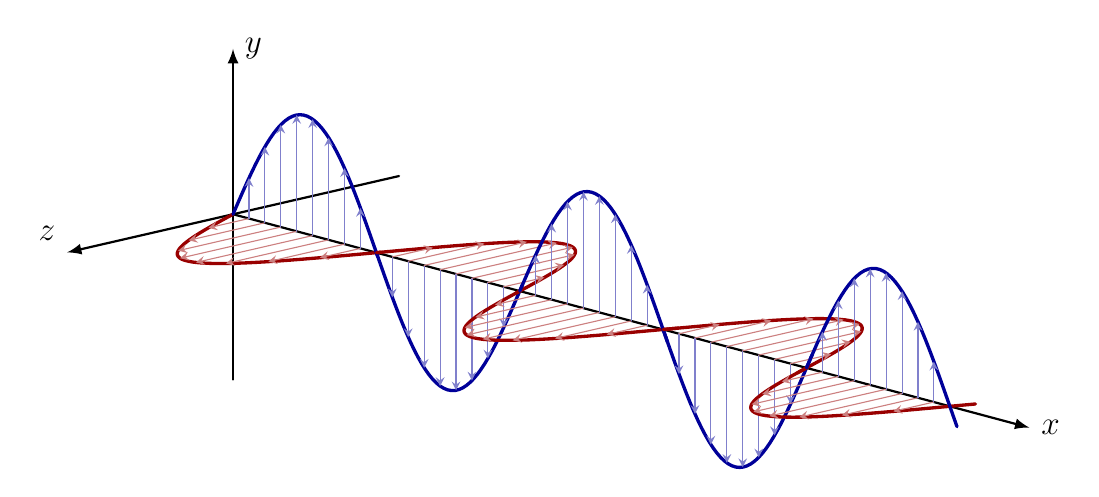
\begin{tikzpicture}[x=(-15:1.2), y=(90:1.0), z=(-150:1.0),
                line cap=round, line join=round,
                axis/.style={black, thick,->},
                vector/.style={>=stealth,->}]
                \large
                \def\A{1.5}
                \def\nNodes{5} % use even number
                \def\nVectorsPerNode{8}
                \def\N{\nNodes*40}
                \def\xmax{\nNodes*pi/2*1.01}
                \pgfmathsetmacro\nVectors{(\nVectorsPerNode+1)*\nNodes}

                \def\drawENode{ % draw E node and vectors with some offset
                    \draw[myblue,very thick,variable=\t,domain=\iOffset*pi/2:(\iOffset+1)*pi/2*1.01,samples=40]
                    plot (\t,{\A*sin(\t*360/pi)},0);
                    \foreach \k [evaluate={\t=\k*pi/2/(\nVectorsPerNode+1);
                    \angle=\k*90/(\nVectorsPerNode+1);}]
                    in {1,...,\nVectorsPerNode}{
                        \draw[vector,myblue!50]  (\iOffset*pi/2+\t,0,0) -- ++(0,{\A*sin(2*\angle+\iOffset*180)},0);
                    }
                }
                \def\drawBNode{ % draw B node and vectors with some offset
                    \draw[myred,very thick,variable=\t,domain=\iOffset*pi/2:(\iOffset+1)*pi/2*1.01,samples=40]
                    plot (\t,0,{\A*sin(\t*360/pi)});
                    \foreach \k [evaluate={\t=\k*pi/2/(\nVectorsPerNode+1);
                    \angle=\k*90/(\nVectorsPerNode+1);}]
                    in {1,...,\nVectorsPerNode}{
                        \draw[vector,myred!50]  (\iOffset*pi/2+\t,0,0) -- ++(0,0,{\A*sin(2*\angle+\iOffset*180)});
                    }
                }

                % main axes
                \draw[axis] (0,0,0) -- ++(\xmax*1.1,0,0) node[right] {$x$};
                \draw[axis] (0,-\A*1.4,0) -- (0,\A*1.4,0) node[right] {$y$};
                \draw[axis] (0,0,-\A*1.4) -- (0,0,\A*1.4) node[above left] {$z$};

                % draw (anti-)nodes
                \foreach \iNode [evaluate={\iOffset=\iNode-1;}] in {1,...,\nNodes}{
                    \ifodd\iNode \drawBNode \drawENode % E overlaps B
                    \else        \drawENode \drawBNode % B overlaps E
                    \fi
                }

            \end{tikzpicture}
        \end{minipage}%
        \begin{minipage}{0.43\textwidth}
            \centering
            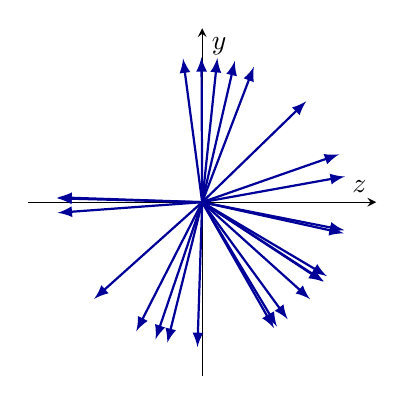
\begin{tikzpicture}
                \begin{axis}[
                axis lines=middle,
                enlargelimits=false,
                height=6cm,
                width=6cm,
                xmin=-1.2, xmax=1.2,
                ymin=-1.2, ymax=1.2,
                xtick=\empty, ytick=\empty,
                xlabel={$z$}, ylabel={$y$}
                ]

                % Number of vectors (adjust as needed)
                \foreach \i in {1,...,25} { % Adjust 25 for more or fewer vectors
                    \pgfmathsetmacro{\angle}{rand*360} % Generate a random angle
                    \pgfmathsetmacro{\x}{cos(\angle)}
                    \pgfmathsetmacro{\y}{sin(\angle)}
                    \addplot[->, thick, myblue] coordinates {(0,0) (\x,\y)};
                }

                \end{axis}
            \end{tikzpicture}
        \end{minipage}
    \end{figure}
    \noindent Most commonly occurring waves such as light are not always two perfect electric and magnetic fields.
    Most waves from the front look like the right graph, where the fields are all oriented randomly.
    The orientation of the electric field is referred to as \textbf{polarization},
    in which the randomly polarized wave is considered unpolarized.
    On the other hand, the wave on the left is vertically polarized.
    We can \textbf{polarize} the light using a polarizing sheet, causing the intensity decreases:
    \begin{equation}
        I = \frac{1}{2} I_0 \tag{one-half rule}
        \end{equation}
    If the light is \textbf{already polarized,} but hits another polarizing sheet,
    we take the polarizing direction into account:
    \begin{equation}
        I = I_0 \cos^2(\theta_f - \theta_i ) \tag{cosine-squared rule}
    \end{equation}

Thest


\end{document}
